\newpage

\subsection{Exercices : récurrence/transience}
\vspace{5mm}
\textbf{Exercice 7.5} [Fonction de Green]

\noindent Allons un peu plus loin dans l’étude de la fonction de Green. Soit $x, y \in E$ deux états. Montrer que :
\begin{enumerate}
    \item Si $x \not\to y$, alors $G(x, y) = 0$.
    \item Si $x \to y$ et
    \begin{itemize}
        \item $y$ est transient, alors $G(x, y) < \infty$ ;
        \item $y$ est récurrent, alors $G(x, y) = \infty$.
    \end{itemize}
    \item La fonction de Green satisfait à l'équation,
    \[
    G = PG + I \quad \Leftrightarrow \quad \forall (x, y) \in E^2, \, G(x, y) = \sum_{z \in E} p(x, z)G(z, y) + \delta_{\{x=y\}}.
    \]
\end{enumerate}

\noindent \textit{Solution de l’exercice 7.5.}\\
\begin{enumerate}
    \item Si \(x \not\to y\), alors pour tout \(n \geq 0, P^{(n)}(x, y) = 0\). Ainsi, d’après le Lemme 7.10, \(G(x, y) = 0\).
    \item On a,
    \[
    x \to y \quad \Leftrightarrow \quad \mathbb{P}_x [T_y < \infty] > 0,
    \]
    (Preuve dans l’Exercice 9.6. de “Exercices de Probabilités”, Cottrell \& al.)\\
    De plus, si y est transient, \(G(y, y) < \infty\) et si \(y\) est récurrent \(G(y, y) = \infty\). En utilisant la deuxième égalité du Lemme 7.12, ceci démontre le point 2.
    \item D’après le Lemme 7.10,
    \begin{align*}
        G(x, y) &= \sum_{n=0}^\infty P^{(n)}(x, y) = P^{(0)}(x, y) + \sum_{n=1}^\infty P^{(n)}(x, y) \\
        &= \delta_{\{x=y\}} + \sum_{n=1}^\infty \sum_{z \in E} p(x, z) P^{(n-1)}(z, y), \quad \text{d'après Chapman-Kolmogorov} \\
        &= \delta_{\{x=y\}} + \sum_{z \in E} p(x, z) \sum_{n=1}^\infty P^{(n-1)}(z, y) = \delta_{\{x=y\}} + \sum_{z \in E} p(x, z) \sum_{n=0}^\infty P^{(n)}(z, y) \\
        &= \delta_{\{x=y\}} + \sum_{z \in E} p(x, z) G(z, y).
    \end{align*}
\end{enumerate}


\noindent\textbf{Exercice 7.6.}
On considère une chaîne de Markov $(X_n)_{n \geq 0}$ d’espace d’état $E = \{1, 2, 3\}$ et de matrice de transition 
\[
P = 
\begin{pmatrix}
0 & 1 & 0 \\
\frac{1}{2} & \frac{1}{2} & 0 \\
\frac{1}{3} & \frac{1}{3} & \frac{1}{3}
\end{pmatrix}.
\]

\begin{enumerate}
    \item Dessiner le graphe associé à cette chaîne de Markov et classifier les états (récurrents/transients).
    \item Calculer la fonction de Green pour toutes les paires de points $(x, y) \in E^2$. En déduire la probabilité de ne jamais revenir en $3$ sachant que l’on est parti de $3$.
\end{enumerate}

\noindent \textit{Solution de l’exercice 7.6.}\\
\begin{enumerate}
    \item Graphe à faire. Les classes d’équivalence sont ${1, 2}$ et ${3}$. La classe ${1, 2}$ est fermée et finie, donc récurrente. La classe ${3}$ permet d’atteindre la classe ${1, 2}$ ; elle n’est pas fermée, donc transiente.
    \item  D’après les points $1$ et $2$ de l’Exercice 7.5, on a que la matrice des coefficients de la fonction de Green est de la forme,

    \[
    G = 
    \begin{pmatrix}
        \infty & \infty & 0 \\
        \infty & \infty & 0 \\
        \infty & \infty & G(3, 3)
    \end{pmatrix}
    \]
\end{enumerate}
\noindent Pour déterminer $G(3, 3)$ on utilise le Point 3 de l’Exercice 7.5 :
\[
G(3, 3) = 1 + \sum^{3}_{z=1}p(z, 3)G(z, 3) = 1 + \frac{1}{3}G(3, 3).
\]

\noindent Ainsi, $\frac{2}{3}G(3, 3) = 1$, autrement dit $G(3, 3) = \frac{3}{2}$. On en déduit la probabilité de ne jamais revenir en $3$ sachant que l’on est parti de $3$ :
\[
\mathbb{P}_3[T_3 = \infty] = \frac{1}{G(3, 3)} = \frac{2}{3}
\]


\noindent \textbf{Exercice 7.7} Classifier les états (récurrents / transients) des exercices du Chapitre 5.3 : Exercice 5.4 (marche aléatoire sur $\mathbb{Z}$), Exercice 5.6 (fort carré), Exercice 5.7 (transmission d’un bit informatique), Exercice 5.9 (ruine du joueur), Exercice 5.10 (plagiste et ses voiliers).\\

\noindent \textit{Solution de l’exercice 7.7.}
\begin{itemize}
    \item Exercice 5.4 (marche aléatoire sur $\mathbb{Z}$). Chaîne irréductible. Il suffit donc de considérer un état. Dans l’Exercice 6.4 on a montré que
\[
\text{Si} \quad p \neq \frac{1}{2}, G(x, x) = \sum_{n=0}^{\infty}P^{(n)}(x,x) < \infty
\]
\[
\text{Si} \quad p = \frac{1}{2}, G(x, x) = \sum^{\infty}_{n=0}P^{(n)}(x, x) = \infty
\]

\noindent Ainsi, la marche aléatoire est récurrente dans le cas symétrique et transiente sinon. Remarquer que dans le cas non symétrique, on a un exemple de classe fermée (infinie) et non-récurrente.
    \item Exercice 5.6 (fort carré) ou marche aléatoire sur $\mathbb{Z}/n\mathbb{Z}$.Chaîne irréductible. Elle est récurrente car finie.
    \item Exercice 5.7 (transmission d’un bit informatique). Chaîne irréductible. Elle est récurrente car finie.
    \item Exercice 5.9 (ruine du joueur). Trois classes : $\{0\}, \{N\}, \{1,..., N-1\}$  Les classes $\{0\}, \{N\}$ consistent en un seul sommet et sont fermées, il s’agit d’états absorbants. La classe $\{1,..., N-1\}$ n’est pas fermée car les classes $\{0\}, \{N\}$ sont accessibles depuis elle. Ainsi les états absorbants sont récurrents et la classe $\{1,..., N-1\}$ est transiente.
    \item Exercice 5.10 (plagiste et ses voiliers). Chaîne irréductible. Elle est récurrente car finie.
\end{itemize}

\noindent \textbf{Exercice 7.8 [Qui perd, perd tout]}

Nous considérons un joueur dont la probabilité de donner une bonne réponse est $p$ quelle que soit la question posée et la probabilité de donner une réponse fausse est $1-p$, avec $0 < p < 1$. Nous supposons que les réponses sont indépendantes les unes des autres et que s’il donne une bonne réponse, il gagne 1, et s’il donne une mauvaise réponse, il perd tout. La richesse de départ est $X_0 = 0$ et, pour tout $n \geq 1$, on note $X_n$ sa fortune à l’instant $n$.
\begin{enumerate}
    \item Montrer qu’il s’agit d’une chaîne de Markov. Donner son graphe et sa matrice de transition.
    \item Montrer que cette chaîne de Markov est irréductible.
    \item Soit $T_0 = \inf\{n > 0 \mid X_n = 0\}$ le temps d’atteinte de $0$. Pour tout $n \in \mathbb{N}^*$, calculer $P_0[T_0 = n]$.
    \item En déduire que la chaîne est récurrente.
\end{enumerate}

\noindent \textit{Solution de l’exercice 7.8.}
\begin{enumerate} 
    \item Le processus $(X_n)_{n \geq 0}$ est à valeurs dans $E = \mathbb{N}$. Soit $Y_n$ la variable aléatoire valant 1 si le joueur répond juste à la n-ième question, et 0 sinon. Alors $(Y_n)_{n\geq 1}$ est une suite de variables aléatoires i.i.d. de loi de Bernoulli de paramètre $p$, indépendante de $X_0$. Pour tout $n \geq 0$, la fortune du joueur à l’instant $n + 1$ est :

\[
X_{n+1} = 
\begin{cases}
X_n + 1 & \text{si } Y_{n+1} = 1 \\
0 & \text{si } Y_{n+1} = 0
\end{cases}
\]
\[
= (X_n + 1) \mathbb{I}_{\{Y_{n+1}=1\}}.
\]
Ainsi d’après l’Exercice 5.5,$ (X_n)_{n \geq 0}$ est une chaîne de Markov.
La matrice de transition $P = (p(x, y))$ a pour coefficients non nuls,
\[
\forall x \in \mathbb{N}, p(x, x+1) = p \quad p(x, 0) = 1 - p.
\]
\newpage
\begin{figure}[h]
\[
P =
\begin{array}{c@{}c@{}c} 
\begin{array}{r}
0 \quad 1 \quad 2 \quad 3 \quad \cdots
\end{array}
\\
\begin{pmatrix}
    1 - p & p & 0 & 0 & \cdots \\
    1 - p & 0 & p & 0 & \cdots \\
    1 - p & 0 & 0 & p & \cdots \\
    1 - p & 0 & 0 & 0 & \cdots \\
    \vdots & \vdots & \vdots & \vdots & \ddots
\end{pmatrix}
&
\begin{array}{r}
0 \\ 1 \\ 2 \\ 3 \\ \vdots
\end{array}

\end{array}
\]
\centering
\caption{Matrice de transition du jeu.}
\end{figure}


\noindent Le graphe associé à cette chaîne de Markov est,
\begin{figure}[h!]
    \centering
    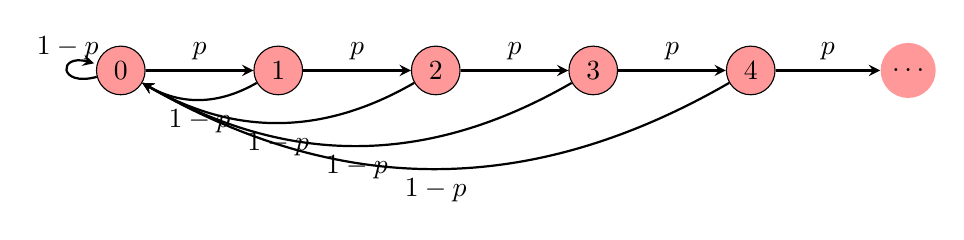
\begin{tikzpicture}[>=stealth, node distance=2cm]
        % Style des noeuds
        \tikzstyle{state} = [circle, draw, fill=red!40, minimum size=0.5cm, node distance=2cm]

        % Définition des noeuds
        \node[state] (0) {0};
        \node[state] (1) [right of=0] {1};
        \node[state] (2) [right of=1] {2};
        \node[state] (3) [right of=2] {3};
        \node[state] (4) [right of=3] {4};
        \node[state, draw=none] (dots) [right of=4] {$\dots$};

        % Arcs entre les noeuds
        \draw[->, thick] (0) edge[loop left] node[above] {$1-p$} (0);
        \draw[->, thick] (0) -- node[above] {$p$} (1);
        \draw[->, thick] (1) -- node[above] {$p$} (2);
        \draw[->, thick] (2) -- node[above] {$p$} (3);
        \draw[->, thick] (3) -- node[above] {$p$} (4);
        \draw[->, thick] (4) -- node[above] {$p$} (dots);
        
        % Backward arrows
        \draw[->, thick, bend left] (1) to node[below] {$1-p$} (0);
        \draw[->, thick, bend left] (2) to node[below] {$1-p$} (0);
        \draw[->, thick, bend left] (3) to node[below] {$1-p$} (0);
        \draw[->, thick, bend left] (4) to node[below] {$1-p$} (0);

    \end{tikzpicture}
    \caption{Graphe de la ruine du joueur.}
\end{figure}

    \item Nous constatons que tous les points communiquent entre eux. En effet, soient deux états $x$ et $y$ :
    \begin{itemize}
        \item Si $y > x$, alors partant de $x$ nous pouvons atteindre $y$ en $y - x$ étapes en gagnant successivement $y - x$ fois : $P^{(x - y)}(x, y) = p^{y - x} > 0$.

        \item Si $y<x$, alors partant de x nous pouvons perdre immédiatement et gagner $y$ fois pour atteindre la fortune $y: P^{(1+y)}(x, y) = (1-p)p^y > 0$.
    \end{itemize}
Il n’y a donc qu’une seule classe et la chaîne est irréductible.\\
\item Soit $n \in \mathbb{N}^*$. Alors,\\

\begin{align*}
    \mathbb{P}_0[T_0=n] &= \mathbb{P}[\{\text{le joueur répond juste aux $(n-1)$ premières questions et faux à la n-ième\}}] \\
    &= \mathbb{P}_0[\{Y_1 = 1, \dots, Y_n-1 = 1, Y_n = 0\}], \text{ d'après Chapman-Kolmogorov} \\
    &= p^{n-1}(1-p), \text{ par indépendance} \\ 
\end{align*}


Ainsi la loi conditionnelle de $T_0$ sachant ${X_0 = 0}$ est une loi géométrique de paramètre $(1-p)$ sur $N^*$

\item On a, 
$$
\mathbb{P}_0[T_0 < \infty] = \sum^{\infty}_{n=1}\mathbb{P}_0[T_0=n] = (1-p)\sum^{\infty}_{n=1}p = \frac{1-p}{1-p} = 1
$$
et la chaîne est donc récurrente.
\end{enumerate}


\noindent \textbf{Exercice 7.9 [Ruine du joueur, suite]}

On reprend l’Exercice 5.9 de la ruine du joueur : deux joueurs $A$ et $B$ disposent d’une fortune initiale de $a$ et $b$ euros respectivement, avec $a, b > 0$. Ils jouent au jeu de hasard suivant : la mise est de 1 euro par partie ; les parties sont indépendantes et à chacune d’entre elles le joueur $A$ a une probabilité $p$ de gagner (et donc $1-p$ de perdre), avec $0 < p < 1$. Le jeu se déroule jusqu’à la ruine d’un des deux joueurs. Notons $N = a + b$, alors la durée du jeu est $T = \inf\{n > 0 \mid X_n \in \{0, N\}\}$. Calculer la probabilité que le joueur $A$ gagne.\\


\noindent \textit{Solution de l’exercice 7.9.} Notons $u(x) = P_x[X_T = N]$, c’est-à-dire la probabilité que le joueur gagne sachant que sa fortune initiale est $x$, avec $x \in \{0, \dots , N\}$. Finalement, on sera intéressé par la probabilité $u(a)$ mais on verra qu’il est utile d’élargir le problème pour le résoudre.\\
Montrons que pour tout $x \in \{1, \dots , N-1\}$, en écrivant $q = 1-p$, $u(x)$ satisfait à l’équation :
$$u(x) = pu(x + 1) + qu(x - 1).$$
En effet, comme $a, b > 0$, on sait que $T \geq 1$. En décomposant sur toutes les valeurs possibles de\\
la chaîne à l’instant 1, on obtient,
\begin{align*}
    u(x) &= \mathbb{P}_x[X_T = N] = \sum_{y \in E} \mathbb{P}_x[X_T = N \mid X_1 = y] \mathbb{P}_x[X_1 = y] \\
    &= \sum_{y \in E} \mathbb{P}_y[X_T = N] \mathbb{P}_x[X_1 = y], \quad \text{(en utilisant la propriété de Markov)} \\
    &= pu(x + 1) + (1-p)u(x-1), \quad \text{(car les autres termes où } \mathbb{P}_x[X_1 = y] = p(x, y) 
    \text{ sont nuls).}
\end{align*}

On a les conditions au bord suivantes,
$$
u(0) = 0, \quad u(N) = 1.
$$

Il s’agit de résoudre une récurrence linéaire d’ordre 2. L’équation caractéristique est :
$$
pz^2 - z + q = 
$$

Ce polynôme a deux racines $z_{1, 2} = 1$, $\frac{p}{q}$ si $p \neq q$ et une racine double $Z_1 = 1$ si $p = q = \frac{1}{2}$. Ainsi,

\begin{itemize}
    \item Si $p \neq q$, la solution générale est de la forme
    $$
    u(x) = \lambda z_1^x + \mu z_2^x = \lambda + \mu(\frac{q}{p})^x.
    $$
    En tenant compte des conditions initiales, on résout pour $\lambda$, $\mu$ et on trouve,
    $$
    u(x) = \frac{1-(\frac{q}{p})^x}{1-(\frac{q}{p})^N}.
    $$

    \item Si $p = q = \frac{1}{2}$, la solution générale est de la for
    $$
    u(x) = (\lambda + \mu x)z^x_1 = (\lambda + \mu x).
    $$
    En tenant compte des conditions initiales, on résout pour $\lambda$, $\mu$ et on trouve,
    $$
    u(x) = \frac{x}{N}.
    $$
\end{itemize}